\chapter{Data reconstruction and selection}
\label{sec:Selection}
The data sample used in this analysis originates from \proton\proton collisions and has been recorded in the years 2011 with a center of mass energy $\sqs = 7 \tev$ and 2012 with $\sqs = 8 \tev$, corresponding to an integrated luminosity of \intlum{3 \invfb}.
This chapter describes and motivates the selection criteria for the reconstruction of the decays \LbToDpmunuX and \LbToLcmunu\footnote{If not stated otherwise, the $\mathcal{CP}$ conjugated decays \decay{\Lbbar}{\Dzb\antiproton\mup\neum} and \decay{\Lbbar}{\Lcbar\mup\neum} are included in those samples}.
As the \Dz and the \Lc are not stable enough to be directly indentified and detected, the subsequent decays \DToKpi and \LcTopKpi have been chosen for their reconstruction.
These decays are good to detect at \lhcb, meaning that one gets a clear signal.
Furthermore, with this choice one ends up with the same final state particles for reconstruction in both signal and normalisation channel, namely \pKpi\mun.
Hence, any inefficiencies due to different interaction of particles with the detector should be avoided, at least to first order.

One experimental difficulty arises due to the semileptonic nature of the signal and normalisation channel:
The neutrino cannot be reconstructed.
Consequently it is not possible to fully reconstruct the \Lb and to get a \Lb mass peak for the distinction between signal and background.
This leads to a high pollution of the data sample with backgrounds.

\section{Reconstruction of the decay \LbToDpmunuX}
The main strategy in the reconstruction process of the decay \LbToDpmunuX is to find events with the signature $\decay{X_{b}}{(\DToKpi) \mun \neumb X}$, where $X_b$ denotes a \bquark-quark containg hadron, first.
Then, the proton track is combined to the \Dz\mun vertex to make a \LbToDpmunuX candidate.
It is apparent that a main source of background will be a \decay{\Bd/\Bp}{\Dz\mun\neumb X} decay, where the proton is randomly combined.
To better understand the selection criteria and the way this \textsc{combinatorial background} is reduced, it might be helpful to have a look at a sketch of a typical \LbToDpmunuX decay in Figure \ref{fig:DecaySketch} left.
\begin{figure}[hptb]
	\centering
	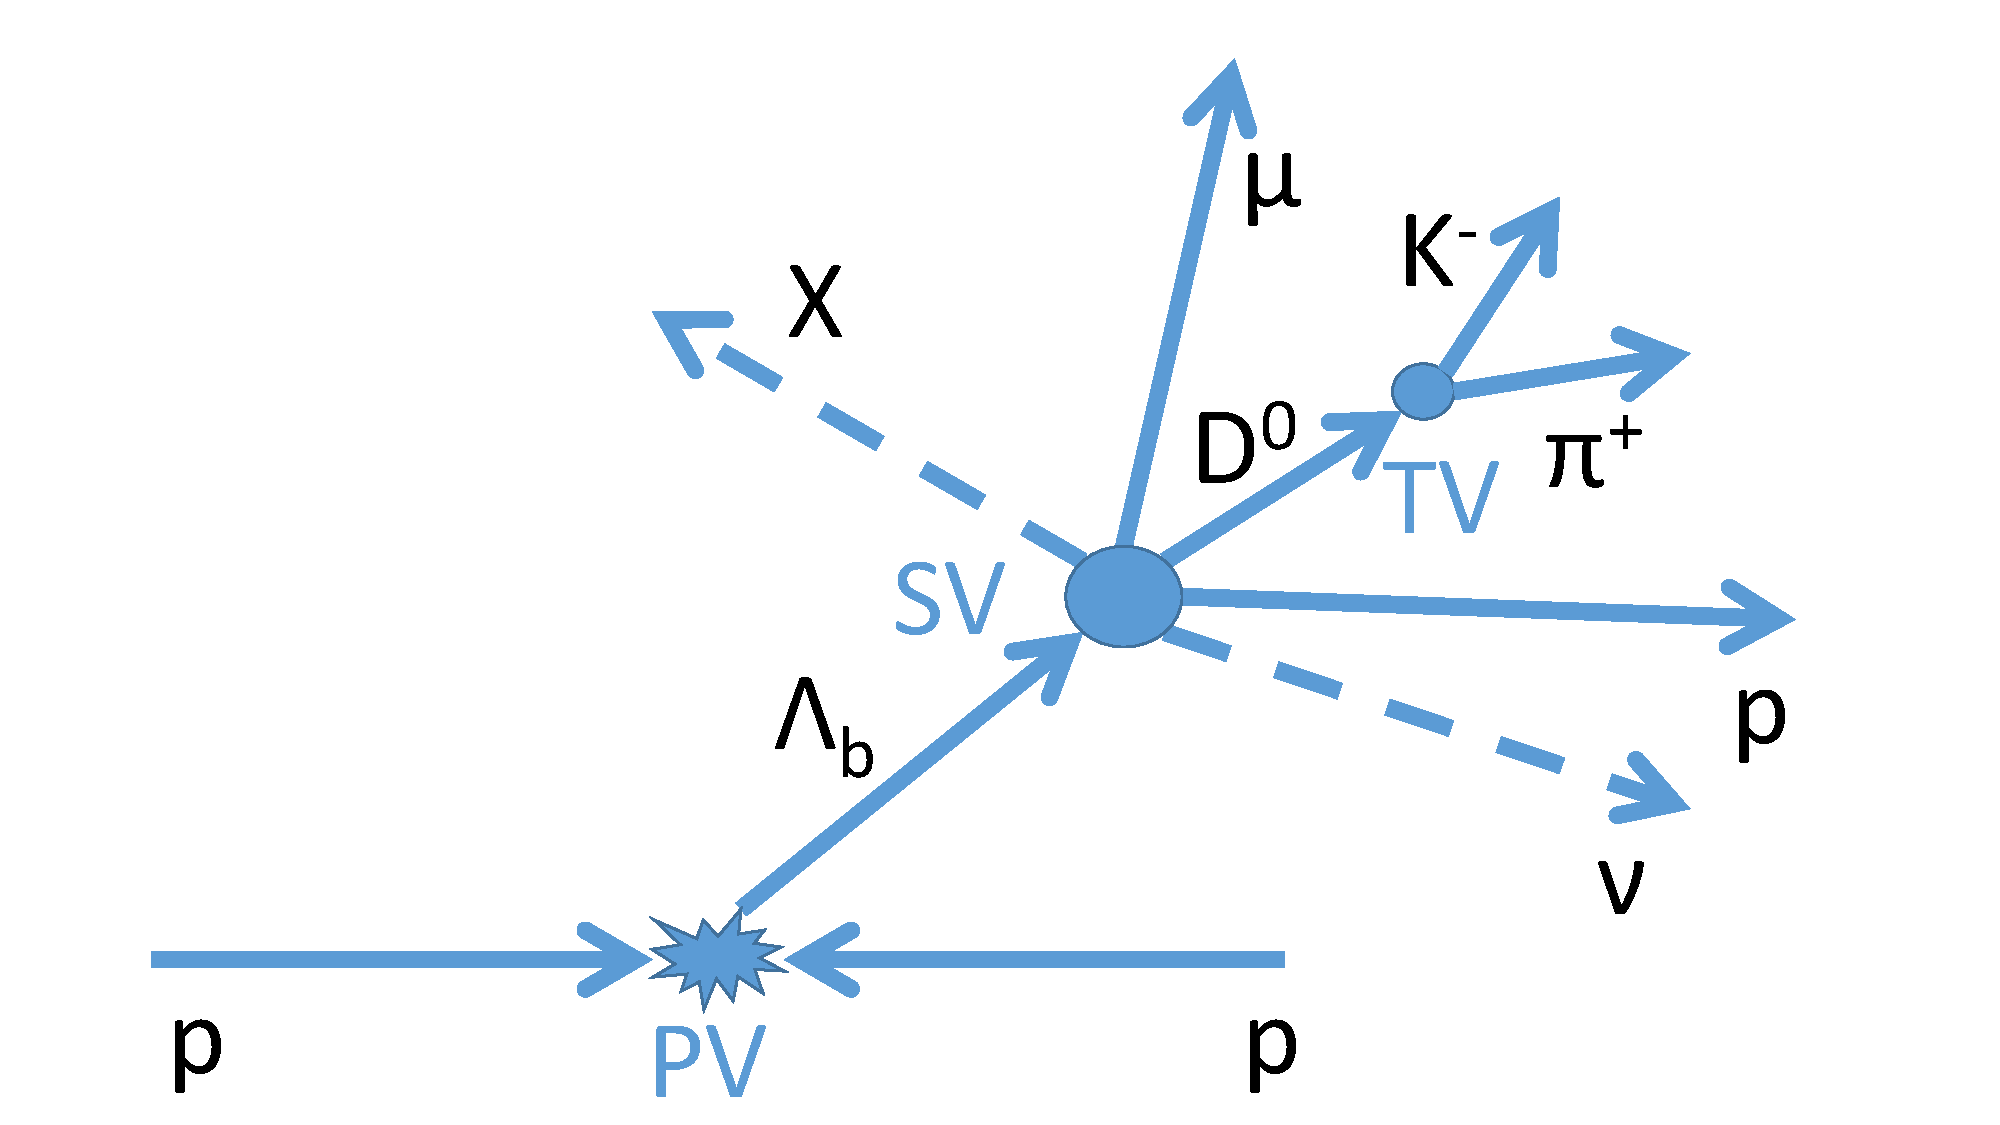
\includegraphics[width=0.49\textwidth]{decay_sketch_signal}
	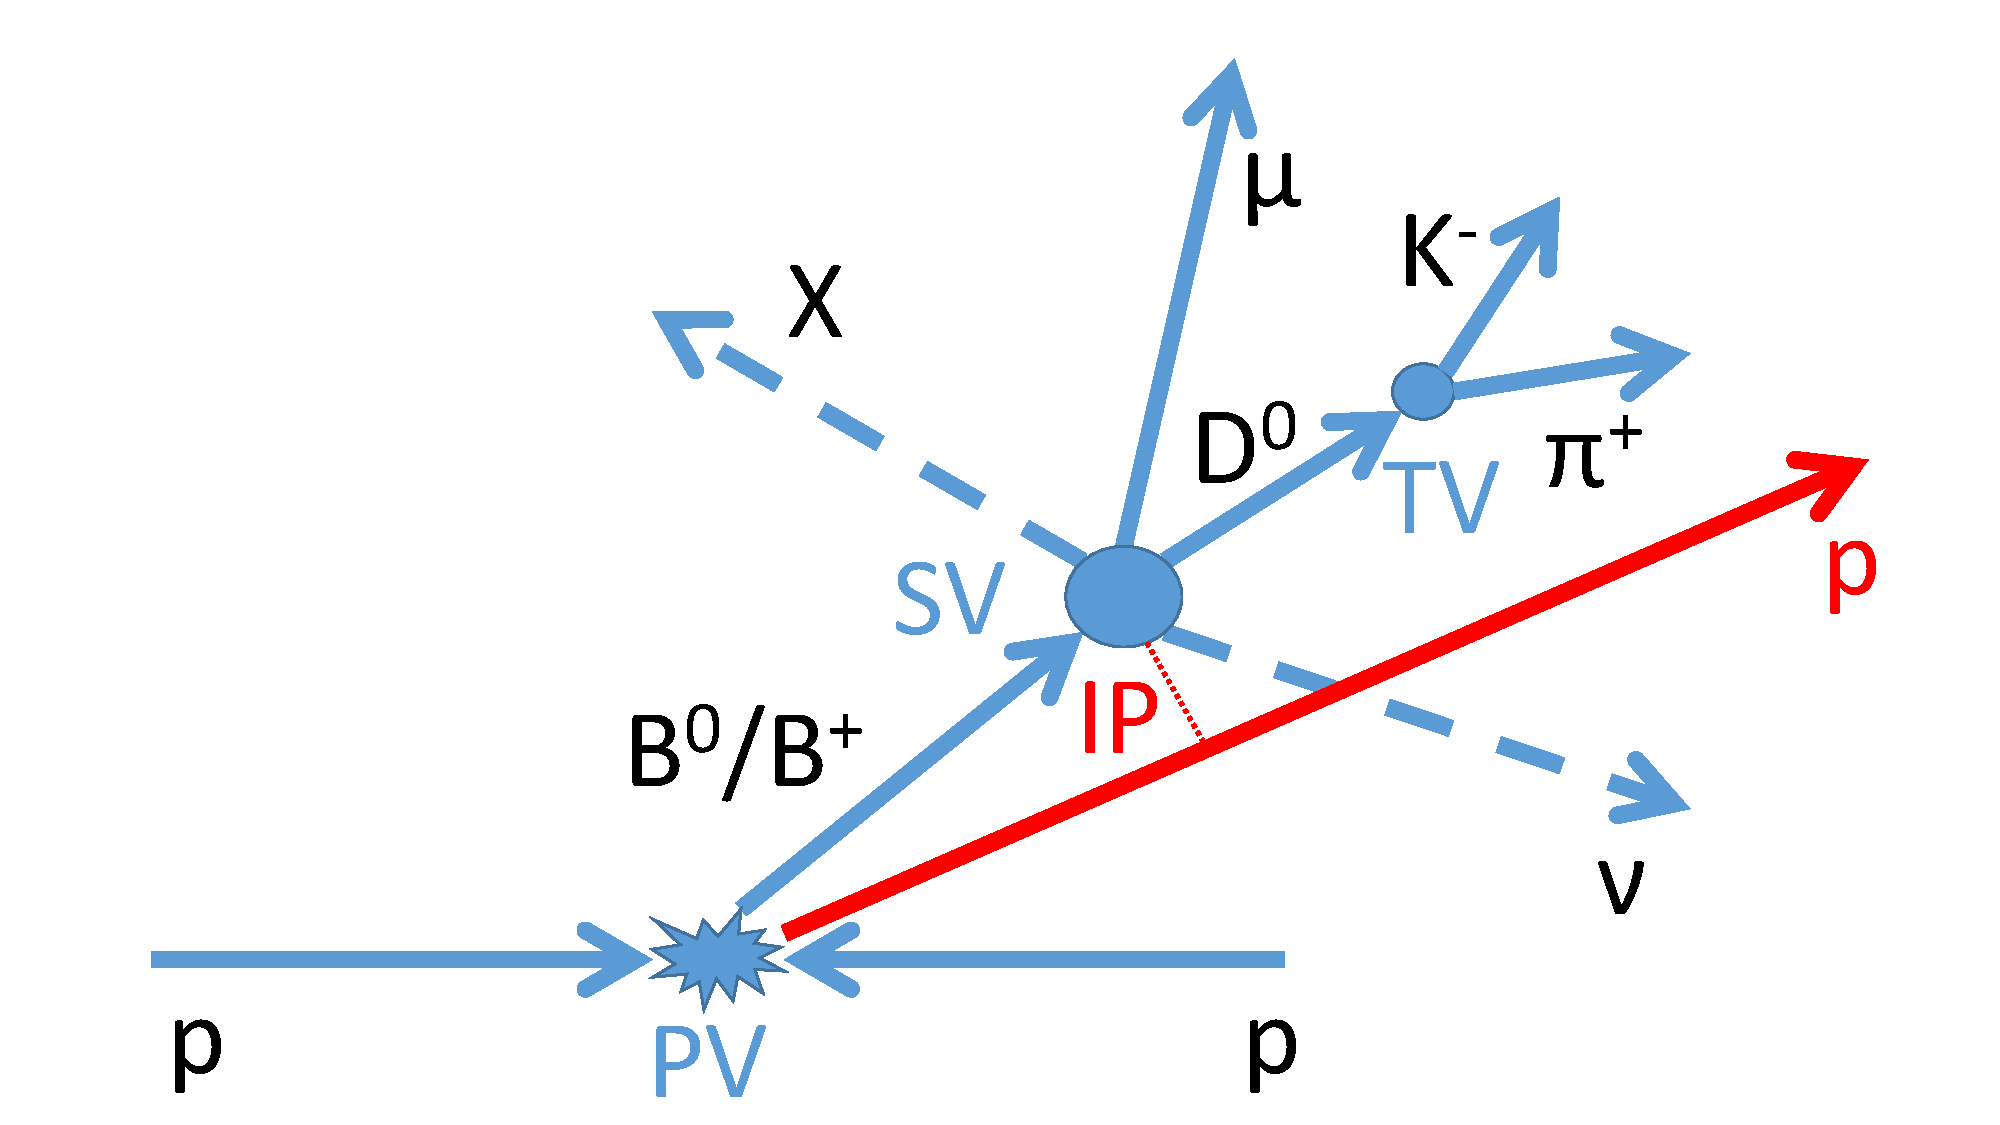
\includegraphics[width=0.49\textwidth]{decay_sketch_background}
	\caption{
        Sketch of the decay topology for a typical \LbToDpmunuX decay (left) and for the background decay \decay{\Bd/\Bp}{\Dz\mun\neumb X} with a randomly combined proton (right).
        In these background events the proton rather poorly makes a vertex with the \Dz\mun candidate, indicated by a large impact parameter (IP).
        Particle tracks drawn with a dashed line are not reconstructed.
        This sketch does neither account for the correct distances between the vertices nor the boost of the particles in $z$-direction.
    }
	\label{fig:DecaySketch}
\end{figure}
Due to its relatively long lifetime, it is typical for a \Lb or in general a \bquark-hadron that it decays at a so called \textsc{secondary vertex (SV)} displaced from the primary \proton\proton interaction, the \textsc{primary vertex (PV)}.
The decay products \Dz, \mun and \proton  originate from the secondary vertex. 
The neutrino and possible further possible particles like pions, denoted as $X$, are not reconstructed.
The \Dz itself lives long enough to decay into a \Km\pip at a \textsc{tertiary vertex (TV)}.

Concerning the combinatrial background \decay{\Bd/\Bp}{\Dz\mun\neumb X} with a randomly combined proton, there is one important difference to the signal.
The proton does not orgin from the secondary vertex but from another source.
It should thus have a significant \textsc{impact parameter (IP)} with respect to the primary vertex.
The impact parameter is defined as the smallest perpendicular distance between a track and a vertex.
An equivalent way is to use the \logIP variable, which will be very important throughout this analysis.
All reconstructed track and vertices are fitted in \lhcb.
From each fit one can retrieve the fit \chisq and the corresponding number of degrees of freedom (ndf).
The \logIP is defined as the logarithm of the difference of the \Dz\mun vertex fit \chisq with and without the proton.
This means the better the proton makes a vertex with the \Dz\mun, the smaller is \logIP and the more likely the event is a real \LbToDpmunuX decay.

\subsection{Reconstruction of the \Dz}
The first step of the reconstruction process is to reconstruct the \Dz.
This is supposed to happen via the \DToKpi signature.
For both, kaon and pion, it is required that their momentum is larger than 2 \gev to ensure that they are not bent out of the detector by the magnet and that the \rich detector gives reliable results on the particle idenitification.
Their transverse momentum is required to be larger than 300 \mev.
This suppresses kaons and pions from the primary interaction, which are usually boosted along the beam pipe, thus having a small transverse momentum.
Aside a good track quality quantified with $\chisqndf < 4$ of the track fit, only tracks with a $\chisqip/\text{ndf} > 4$ are selected, meaning the kaons and pions are not coming from the primary interaction.
\lhcb's particle identification system provides a likelihood for a particle hypothesis of each particle candidate.
For the pion candidate a likelihood is available that it is really a pion or that is a kaon and so on.
One defines the PIDx variable of a particle candidate, which denotes the difference of the logarithmic likelihoods between the hypotheses that this particle is of species x and a pion.
The higher PIDx the more likely the candidate is really a particle x\footnote{Throughout this thesis x is either mu for muons, p for protons and K for kaons.}.
For the kaon candidate a PIDK $>4$ and for the pion candidate a PIDK $<10$ is required.
These two candidates and their tracks are now combined to a \Dz candidate with a good vertex quality of \chisqvtx/ndf $<6$.
Another variable one defines for the reconstruction is DIRA.
It is defined as the cosine of the angle $\alpha$ between the track of a particle and its momentum.
If the detector resolution was perfect, DIRA would be one ($\alpha = 0$) for a signal decay.
Requiring a DIRA close to one ensures that the assigned momentum and track match to each other.
In this case events with a DIRA $>0.99$ of the \Dz are selected.
As last requirement one suppresses combinatorial background by restricting the \Dz to be close to its mean mass, i.e. the mass difference to the PDG value is smaller than 25 \mev and to require a minimum \Dz flight distance with respect to the primary vertex of 5 \mm.

\subsection{Reconstruction of the \Dz\mun candidate}
Having reconstructed the \Dz candidate one needs a muon track to combine them.
The motivation for the requirements on the muon track is analagous to the kaon and pion for the \Dz reconstruction.
Thus they will be just briefly mentioned:
The muon is required to have a minimum transverse momentum of 1.2\gev and a minimum momentum of 6\gev.
The track \chisqndf is smaller than 4 and the \chisqip with respect to the primary vertex larger than 9.
PIDmu is required to be greater than 0.3.
It might happen, that several hits in the detector are incidentally combined to a track albeit coming from different tracks.
The so called ghost probablity gives a measure of this issue and is required to be less than 0.5 for the muon track.

For the combination of \Dz and \mun the vertex shall be again of good qualitiy, i.e. \chisqvtx/ndf $<3$.
To avoid completely random combinations the invariant \Dz\mun mass is required to be between 2.2 and 8.0 \gev and a minimum transverse momentum of 3 \gev.
The minimum DIRA of the \Dz\mun candidate is 0.999.
With a requirement on the flight distance \chisq to be greater than 25 it is ensured that the \Dz\mun decay vertex is certainly displaced form the primary vertex.

\subsection{Reconstruction of the \Lb / \Dz\mun\proton candidate}
The proton's momentum and transverse momentum is required to be 15 \gev and 1 \gev for a good particle identification and to exclude protons boosted from the primary interaction.
To reduce the amount of fake protons, i.e. pions or kaon that are misidentified as protons, tight particle idenitification requirements are applied: PIDp $> 10$ and PIDp$-$PIDK $> 10$.
The \chisqip


\section{Reconstruction of the decay \LbToLcmunu}

\section{Simulation samples}


\textbf{Here begins the old part, which will be rewritten!} \\

The analysis of the decays \LbToDpmunuX (signal channel)  and \LbToLcmunu (normalization channel) requires the reconstruction and selection of possible signal candidates.
The term ``signal candidates" implies, that a data sample doesn't contain only the desired signal events after reconstruction and selection, but is also polluted by events from different sources, albeit looking like signal.
These backgrounds can have several reasons: 
One possibility is that the final state particles are randomly combined but fulfil all the applied criteria. 
This kind of background is also known as combinatoric background.
There are furthermore the so-called physical backgrounds.
With this term one summarises physical decays where one either misidentifies a final state particle or only partially reconstruct an event und thus leading to a wrong interpretation of the decay.
As an example for the misidentification consider the decay \decay{\Lb}{\Dz\proton\pim}. If the \pim is now misidentified as a muonthis decay looks exactly like the signal channel of this analysis.
Partially reconstructed events play an important role in the normalisation channel \LbToLcmunu.
There exists also semileptonic \Lb decays into excited \Lcstar states, \decay{\Lb}{\Lcstar\mun\neumb}.
Subsequently, these excited \Lcstar states decay into an \Lc and additional pions or photons.
If one misses these pions and photons the decay looks exactly like \LbToLcmunu.

Since such misidentified decays or combinatoric backgrounds distort the measurement of physical quantities, the event reconstruction and above all the selection aims to reduce these backgrounds as much as possible while keeping as much signal as possible.
At \lhcb, this procedure is done in several steps, described for the present analysis in this chapter, namely the Trigger, the preselection (or stripping) and the offline selection. 
Nonetheless not every background source can be easily eliminated. 
The handling of such issues is part of chapter \ref{sec:Backgrounds}.

\section{Trigger requirements}
Trigger requirements are already applied during data taking to reduce the arising data to a recordable amount.
There exists so called trigger lines for different physics purposes. 
These trigger lines then contain the requirements on the particles' properties.

Due to their large lifetime and their little interaction with matter muons leave a very clean signal in the detector and are the best suited to trigger on. For the \LbToDpmunuX channel the muon has pass the \texttt{L0Muon\_TOS} line at L0 level. TOS is the abbreviation for Trigger On Signal, i.e. the presence of the signal is sufficient to generate a positive trigger decision \cite{Tolk:1701134}. 
To record an event this line requires that the transverse momentum of at least one muon candidate is larger than 1760\mev\footnote{This requirement changed between 2011 and 2012. For a better readability only the 2012 trigger settings are described here. The 2011 configuration can be found in \cite{Trigger_2011_2012}.}.
At Hlt1 the \texttt{Hlt1TrackMuon\_TOS} line requires the muon candidate to have at least one hit in the VELO and triggers on the track quality.
The full event reonstruction is available at Hlt2 level.
Here, the so called topological trigger lines dedicated to trigger inclusive 2,3 or 4 body decays of \B mesons are applied.
Additionally to kinematical information they are applying requirements on the vertex quality demanding the tracks to be very close to each other.
These trigger lines deliver events containing a \Dz\mun candidate.
These events are afterwards combined with \proton tracks to form a \LbToDpmunuX candidate.

\section{Preselection / Stripping}
The stripping selection serves for the reduction of data in the analysis given a certain decay topology.
The requirements made for a specific decay category are collected in so called stripping lines.
For the \LbToDpmunuX channel the line \texttt{b2D0MuXB2DMuNuXLine} and for \LbToLcmunu the line \texttt{b2LcMuXB2DMuNuXLine} is used.
These lines are dedicated to filter the data for inclusive decays of \bquark containing hadrons to either a \Dz\mun or a \Lc\mun, namely $X_{\bar{b}} \rightarrow (D^0 \rightarrow K^- \pi^+) \mu^- \bar{\nu}_{\mu} X$ or respectively $X_{\bar{b}} \rightarrow (\Lambda_c^+ \rightarrow K^- \pi^+ p^+) \mu^- \bar{\nu}_{\mu} X$.
The requirements included in these lines are mentioned in tables \ref{tab:cuts_D0p} and \ref{tab:cuts_Lc}.
In the following the used variables will be explained.
\begin{itemize}
    \item \ptot (\pt) denotes the total (transverse) momentum of a particle
    \item \textbf{GhostProb:} It might happen, that several hits in the detector are incidentally combined to a track albeit having different sources. 
          A measure how likely such a ``ghost" is, is given by the ghost probability.
    \item The \textbf{impact parameter (IP)} is defined as the smallest perpendicular distance between a track and a vertex, in most cases this is the primary vertex.
    \item As tracks and vertices are fitted, \textbf{\chisq} values can be derived from them. 
          The \textbf{\chisqip} denotes the difference of a vertex fit \chisq value with and without a specific particle. 
          It is thus a measure how well a particle makes a vertex. 
          Requiring a high \chisqip of a particle for instance with respect to the primary vertex ensures that this particle comes from another source.
    \item The particle identification system delivers a likelihood for each particle hypothesis.
          \textbf{PIDx} (or often also \textbf{DLL$_x$}) denotes the difference of the logarithmic likelihoods between the hypothesis that a particle is x and the hypothesis to be a pion.
          The higher PIDx the more likely it is particle x.
    \item \textbf{DIRA} denotes the cosine of the angle between the momentum of the particle and the direction of flight from the primary vertex to the decay vertex.
\end{itemize}

\section{Additional analysis selection}
To further reduce backgrounds prominent in this analysis an additional analysis selection is applied on top of the stripping.
The requirements at this level are also listed in table \ref{tab:cuts_D0p} for the \LbToDpmunuX channel and \ref{tab:cuts_Lc} for \LbToLcmunu.
Some of the requirements are just tightened a bit, but also some further observables are used.

Concerning the \LbToDpmunu channel a high focus has been put on avoiding backgrounds where a kaon or pion is misidentified as a proton. 
For this purpose the particle identification variables have to fulfil the conditions PIDp $> 10$ and PIDp$-$PIDK $> 10$.
Due to the missing neutrino the \Lb mass can't be fully reconstructed.
Thus, only a loose selection can be made by this variable.
It is demanded to be less than 5500 \mev which is less than the actual \Lb mass.
Events peaking around the \Lb mass should be clearly background from particles misidentified as muon.
More on this can be found in section \ref{sec:BKG_misIDmu}.
A way of using more information on the masses is the use of the corrected \Lb mass, which peaks around the \Lb mass if the missing particle (as the missing neutrino here) is massless.
It is thus required to be between 5 and 6 \gev.
Another source of background might be prompt \Dz, i.e. \Dz directly coming from the primary interaction, with a randomly combined muon.
To suppress such events it is required that the combined \Dz\mun particle flies a distinct path and is well separated from the primary vertex.
A measure for this purpose is the flight distance \chisq with respect to the primary vertex, which should be larger than 25.
Except for the twodimensional signal fit where the \logIP distribution is used to distinguish nonresonant signal and background it is required to be less than 1 to eliminate random combinations of protons with the \Dz\mun candidate.
\begin{table}[h]
    \centering
    \caption{Selection requirements for the decay \LbToDpmunuX.}
    \label{tab:cuts_D0p}
    \resizebox{\textwidth}{!}{
    \begin{tabular}{r|lll}
        \hline
                & Variable          & Stripping & Analysis \\
        \hline
        Event   & nLongTracks       & $< 250$   & -- \\
        \hline
        Trigger
        & L0    & --                                & Muon is L0Muon\_TOS \\
        & Hlt1  & B is TOS on any Track line        & Muon is Hlt1TrackMuon\_TOS \\
        & Hlt2  & B is Hlt2Topo(2$|$3$|$4)Body\_TOS & -- \\
        \hline
        Muons
        &  \pt                        & $> 1.2 \gev$    & --\\
        &  \ptot                      & $> 6 \gev$      & --\\
        &  GhostProb                  & $< 0.5$         & -- \\
        &  track \chisq/ndf           & $< 4$           & -- \\
        &  \chisqip w.r.t. PV         & $> 9.0$         & -- \\
        &  PIDmu                      & $> 0.0$         & $> 0.3$ \\
        \hline
        $D^0 \to K^-\pi^+$
        & Daughter $p$                & $> 2 \gev$      & -- \\
        & Daughter \pt                & $> 300.0 \mev$  & -- \\
        & Daughter GhostProb          & $< 0.5$         & -- \\
        & Daughter track \chisq/ndf   & $< 4$           & -- \\
        & Daughter \chisqip w.r.t. PV & $> 4.0$         & -- \\
        & Daughter ($K$) PIDK         & $> 4.0$         & -- \\
        & Daughter ($\pi$) PIDK       & $< 10.0$        & -- \\
        & \chisqvtx/ndf               & $< 6$           & -- \\
        & DIRA w.r.t. PV              & $> 0.99$        & -- \\
        & Mass diff. to PDG           & $< 80 \mev$     & $< 25 \mev$ \\
        & Flight distance w.r.t. PV   & --              & $> 5 \mm$ \\
        \hline
        $D^0\mun$
        & Mass                            & $\in \left[2.2, 8.0\right] \gev$ & -- \\
        & \chisqvtx/ndf                   & $< 6$                            & $< 3 $ \\
        & DIRA w.r.t. PV                  & $> 0.999$                        & -- \\
        & Flight distance \chisq w.r.t. PV& --                               & $ > 25 $ \\
        & Transverse momentum             & --                               & $ > 3000 \mev $ \\
        \hline
        $D^0\mun\proton$
        & $\arccos$(DIRA) w.r.t. PV       & --                               & $ < 0.015 $ \\
        & Mass                            & --                               & $ < 5.5 \gev $\\
        & Corrected Mass                  & --                               & $ \in \left[5, 6\right] \gev $\\ 
        \hline
        \proton
        & \chisqip w.r.t. PV              & -- & $ > 25 $ \\
        & PIDp$-$PIDK                     & -- & $ > 10 $ \\
        & PIDp                            & -- & $ > 10 $ \\
        & Momentum                        & -- & $ > 15 \gev $\\
        & Transverse momentum             & -- & $ > 1 \gev $\\
        & \logIP w.r.t. \Dz\mun vertex  \footnote{not included in twodimensional \Dz\proton signalfit (see section \ref{sec:Signalfit}} & -- & $ < 1 $ \\
        \hline
    \end{tabular}}
\end{table}

Moving on to \LbToLcmunu, the requirements on the proton coming from the subdecay \LcTopKpi are chosen to be the same as in \LbToDpmunuX to avoid different efficiencies due to different selections.
It is furthermore ensured that the \Lc vertex is displaced from the primary interaction by the requirements on the impact parameter and again the flight distance \chisq.
\begin{table}[h]
    \centering
    \caption{Selection requirements for the \LbToLcmunu channel.}
    \label{tab:cuts_Lc}
    \resizebox{\textwidth}{!}{
    \begin{tabular}{r|lll}
        \hline
                & Variable          & Stripping & Analysis \\
        \hline
        Event   & nLongTracks       & $< 250$   & -- \\
        \hline
        Trigger
        & L0    & --                                & Muon is L0Muon\_TOS \\
        & Hlt1  & B is TOS on any Track line        & Muon is Hlt1TrackMuon\_TOS \\
        & Hlt2  & B is Hlt2Topo(2$|$3$|$4)Body\_TOS & -- \\
        \hline
        Muons
        &  \pt                        & $> 1 \gev$      & --\\
        &  \ptot                      & $> 6 \gev$      & --\\
        &  GhostProb                  & $< 0.5$         & -- \\
        &  track \chisq/ndf           & $< 4$           & -- \\
        &  \chisqip w.r.t. PV         & $> 9.0$         & -- \\
        &  PIDmu                      & $> 0.0$         & $> 0.3$ \\
        \hline
        \LcTopKpi
        & Daughter $p$                & $> 2 \gev$      & -- \\
        & Daughter \pt                & $> 250.0 \mev$  & -- \\
        & Daughter GhostProb          & $< 0.5$         & -- \\
        & Daughter \chisqip w.r.t. PV & $> 4.0$         & -- \\
        & Daughter (\proton) PIDp     & $> 0.0$         & $> 10$ \\
        & Daughter (\proton) PIDp-PIDK& --              & $> 10$ \\
        & Daughter (\proton) \ptot    & $> 9 \gev$      & $> 15 \gev$ \\
        & Daughter (\proton) \pt      & --              & $> 1 \gev$ \\
        & Daughter (\proton)\chisqip w.r.t. PV & $> 4.0$& $> 25 $    \\
        & Daughter ($K$) PIDK         & $> -5.0$        & -- \\
        & Daughter ($\pi$) PIDK       & $< 20.0$        & -- \\
        & \chisqvtx/ndf               & $< 6$           & $< 3$ \\
        & DIRA w.r.t. PV              & $> 0.99$        & -- \\
        & Mass diff. to PDG           & $< 80 \mev$     & -- \\
        & \pt                         & $>2.1 \gev$     & -- \\
        & $\log_{10}$(IP) w.r.t. PV   & --              & $ > - 1.5 $ \\
        & Flight distance \chisq w.r.t. PV   & --       & $> 25$ \\
        \hline
        \Lc\mun
        & Mass                            & $\in \left[2.2, 8.0\right] \gev$ & -- \\
        & \chisqvtx/ndf                   & $< 6$                            & -- \\
        & DIRA w.r.t. PV                  & $> 0.999$                        & -- \\
        \hline
    \end{tabular}}
\end{table}

After application of all these requirements there are in total 21444 \LbToDpmunuX (34760 without \logIP cut) and 2670999 \LcTopKpi candidates left for the fits and the further analysis. 
